\documentclass{article}

%% Language and font encodings
\usepackage[english]{babel}
\usepackage[utf8x]{inputenc}
\usepackage[T1]{fontenc}
\usepackage[numbers]{natbib}
\bibliographystyle{plainnat}
\usepackage{booktabs}

%% Sets page size and margins
\usepackage[a4paper,top=3cm,bottom=2cm,left=3cm,right=3cm,marginparwidth=1.75cm]{geometry}

%% Useful packages
\usepackage{amsmath}
\usepackage{amssymb}
\usepackage{graphicx}
\usepackage[colorlinks=true, allcolors=blue]{hyperref}
\usepackage{setspace}
\usepackage{lineno}  % For reviewers
\usepackage{authblk}
\usepackage{blindtext}
\usepackage{fancyhdr}

% Use pretty font
\usepackage[scaled]{palatino}
\renewcommand\familydefault{\sfdefault} 
\usepackage[T1]{fontenc}

% big letter
\usepackage{lettrine}

\pagestyle{fancy}
\rhead{Homeostasis and oscillations}

% -----------------------------------------------------
% -----------------------------------------------------
% -----------------------------------------------------
\title{Homeostatic mechanisms may shape the type and duration of oscillatory modulation.}
\author[1,2,*]{Erik J. Peterson}
\author[2,3,4]{Bradley Voytek}

\affil[1]{Department of Psychology. Carnegie Mellon University, Pittsburgh, PA 15213}
\affil[2]{Department of Cognitive Science,~~~~~~~~~~~~~~~~~~~~~~~~~~~~~~~~~~~~~~~~~~~~~~~~~~~~~~~~~~~~~~~~~~~~~~}
\affil[3]{Neurosciences Graduate Program,~~~~~~~~~~~~~~~~~~~~~~~~~~~~~~~~~~~~~~~~~~~~~~~~~~~~~~~~~~~~~~~~~~~~}
\affil[4]{Hal{\i}c{\i}o\u{g}lu Data Science Institute, University of California, San Diego, 92093~~~~}
\affil[*]{Corresponding author: Erik.Exists@gmail.com~~~~~~~~~~~~~~~~~~~~~~~~~~~~~~~~~~~~~~~~~~~~~~~~~~}
\date{}                     %% if you don't need date to appear
\setcounter{Maxaffil}{0}
\renewcommand\Affilfont{\itshape\small}


\begin{document}
\maketitle
\linenumbers
% -----------------------------------------------------
% -----------------------------------------------------
% -----------------------------------------------------
\begin{abstract}
Neural oscillations are observed ubiquitously in the mammalian brain, but their stability is quite variable. Some oscillations are \textit{tonic} and last for seconds or even minutes. Others oscillations are unstable. They appear for only as a single-cycle \textit{burst}. Likewise, some oscillations rely on excitatory AMPAergic synapses, but others are GABAergic and inhibitory. Why both kinds of diversity are present is not known. We hypothesized Ca$^{2+}$-dependent homeostasis is important to finding an explanation. We tested this in a highly simplified model of hippocampal neurons. In this model homeostasis can profoundly alter the modulatory effect of neural oscillations. Under homeostasis, tonic AMPAergic oscillations actually \textit{decrease} excitability and desynchronize firing. Tonic oscillations that are synaptically GABAergic--like those in real hippocampus--don't provoke a homeostatic response, however. If our simple model is correct, homeostasis can explain why the theta rhythm in hippocampus is synaptically inhibitory: GABA has little to no intrinsic homeostatic response, and so can preserve a cell's dynamic range under tonic oscillation. Based on these results we also speculate that homeostasis can explain why AMPAergic oscillations in cortex often appear as bursts. Bursts minimally interact with the slow homeostasis time constant, and so retain their excitatory effect.\\
\end{abstract}

% -----------------------------------------------------
% -----------------------------------------------------
% -----------------------------------------------------
\noindent
\textsc{\textbf{New and Noteworthy}} The intricate interplay of neuromodulators, like acetylcholine, with homeostasis is well known. The interplay between oscillatory modulation and homeostasis is not. We studied oscillatory modulation and intrinsic homeostasis for the first time in a simlified model of hippocampal neurons. We report a paradoxical result: Ca\textsuperscript{2+}-mediated homeostasis causes normally synchronizing AMPAergic oscillations to become inhibitory and desynchronizing. This result, along with other new observations, suggests homeostasis might be just as complex -- and just as important -- for oscillations as it is for all other kinds of modulation.

\section*{Introduction}
\lettrine[loversize=0,nindent=0,realheight=true]{N}{} euromodulation and homeostasis are inter-linked but opposing phenomena. Modulation perturbs excitability, which we define as the propensity for a stimulus to elicit an action potential. Homeostasis acts to quench this perturbation, driving the excitability of the cell back to a biologically desirable set point \cite{LeMasson1993,Abbott1993}. While the interplay between chemical modulators and homeostasis has been studied for more than 20 years \cite{LeMasson1993,Abbott1993,Golowasch1999,Marder2014,Marder2015,Gutierrez2013}, the relationship between population-level synaptic modulations--like neural oscillations--and homeostasis is not well understood, on either theoretical or empirical grounds. Like neuromodulators, neural oscillations alter excitability and firing statistics. Uniquely though, oscillations can group action potentials into synchronous windows of activity \cite{Lisman2013,Voytek2015}. Grouping action potentials can improve signal to noise and increase the number of coincident firing events \cite{Chen2013,Zhou2015,Voytek2015a,Peterson2017}, which drives learning at individual synapses \cite{Muller2011,Song2000,Markram1997}. 

We propose the same mechanisms that link homeostasis with chemical neuromodulation can also come into play with oscillatory modulation. After all, both kinds of modulation lead to tonic changes in spiking and, as a result, changes in Ca\textsuperscript{2+} concentration \cite{Liu1998}. 

To test this, we model activity-dependent intrinsic homeostasis in a feed-forward population of hippocampal pyramidal cells \cite{Siegel1994}. By feed-forward we mean there are no lateral or recurrent connections in the population. Firing activity is driven only by afferent synaptic input, and homeostasis is mediated by a Ca\textsuperscript{2+}-dependent mechanism \cite{Golowasch1999,Marder2014,Marder2015,Gutierrez2013,OLeary2014} pioneered by LeMasson \cite{LeMasson1993,Abbott1993}. Here Ca\textsuperscript{2+} acts a sensor for tonic changes in the membrane voltage. To counter tonic changes in Ca\textsuperscript{2+} levels, the expression of ion channels is altered, returning the Ca\textsuperscript{2+} level to a predefined ``good'' value \cite{Golowasch1999,OLeary2013}. Following Siegel \cite{Siegel1994}, increases in Ca\textsuperscript{2+} lead to downregulation of Na\textsuperscript{+} and Ca\textsuperscript{2+} channels, and upregulation of fast K\textsuperscript{+} channels. To minimize the effect of homeostasis on the rise and fall of action potential dynamics, we also add a KCa channel which is not present in Siegel \citep{Siegel1994}. In real cells intrinsic homeostasis changes the expression level of ion channels \cite{OLeary2013}. Here, these details are not directly simulated. Instead we mimic the net or bulk effect of all ion channels using a single equation \cite{LeMasson1993,OLeary2013,OLeary2014}.

Given chemical modulators operate on both short and long times scales \cite{Marinelli2014,Marder2014,Cohen2015,Daw2002}, we examined two timescales of oscillatory modulation. We contrast the effects of short 4-cycle bursts of oscillation to long lasting tonic rhythms. Both are observed {\textit{in vivo}}, and are known to play different physiological, cognitive, and computational roles \cite{Lundqvist2016,vanEde2018,Peterson2017}. We also explore synapse type, examining both AMPA- or GABA-ergic oscillations. 

% \textit{Bursts} of excitation don't show homeostatic suppression. They are two fast for the slow Calcium sensor to detect. Inhibitory GABAergic also have little to no homeostatic effect, suggesting that inhibitory oscillations might better isolate any phase coding scheme from the stimulus-driven response. This is might be important, for example, in hippocampal phase-coding schemes of memory \cite{Lisman2013}. 

% -----------------------------------------------------
% -----------------------------------------------------
% -----------------------------------------------------
\section*{Results}
We assessed the impact of homeostasis in a simple model that received oscillatory inputs that are either transiently bursting, or tonic. We found that increasing the strength of AMPAergic oscillatory inputs resulted in a homeostatic response that, when reaching an appropriate level of average calcium, overcompensates to actually suppresses the postsynaptic neuron's spiking. That is, paradoxically, an increase in drive when combined with homeostasis results in a decreased response. 

Specifically, we study Ca\textsuperscript{2+}-mediated homeostasis in a feed-forward population of 100 Hodgkin-Huxley neurons. By feedforward we mean neurons in the population are driven only by the inputs to the model. Cells have no lateral or recurrent connections. We modulate this population with neural oscillations. Oscillations are modelled as a set of 1000 Poisson neurons. To change the level of oscillatory modulation strength, we alter the firing rate of the Poisson population. Average synaptic strengths were fixed, but drawn from a uniform distribution for each simulation (see \textit{Methods}). An oscillation's temporal duration was simulated as either tonic, which lasted for the entire experiment, or as a 4-cycle burst. Bursts were delivered only at the end of a trial, where they overlap with the input stimulus (Figure~\ref{fig:f1}\textbf{a}). The stimulus input was also drawn from a 1000 cell Poisson population. It lasted 0.5 seconds, and had an average firing rate of 6 Hz. The stimulus was fixed for all experiments, and was delivered only once homeostatic equilibrium was reached \cite{Barth2012} (Figure~\ref{fig:f1}). During the stimulus window we measured the population's firing rate and synchrony. It is these numbers we report throughout.

Each experiment began with an instantiation of a randomly generated population. A single example neuron is depicted in Figure~\ref{fig:f1}\textbf{b}. This population is subjected to a range of modulatory and control conditions, including oscillatory strength, duration, and synapse type (AMPA or GABA). Each experiment lasted 20 seconds. In Figure~\ref{fig:f1}\textbf{c} we depict key aspects of model output during an experiment. 

After homeostatic equilibrium is reached, we measure two features: the synchrony between action potentials (measured by the Kappa correlation) and changes in the excitability of the system (measured as a change in population firing rate). Both of these measures are defined in the \textit{Methods}. To ensure a consistent comparison between experiments, measurements were made over the same 4-cycle or 0.5 second period in all simulations. Source code for all simulations is available at \url{https://github.com/voytekresearch/resistingrhythm}

The homeostatic response in our simple model decreases the sodium conductance and increases the potassium conductance (Figure~\ref{fig:f1}\textbf{c}, \textit{bottom panel}). Combined these make it harder for the model cell to generate action potentials. This basic mechanism explains the loss of excitability in some conditions of our model and, in turn, the desynchronization of population activity. 

\begin{figure}
\centering
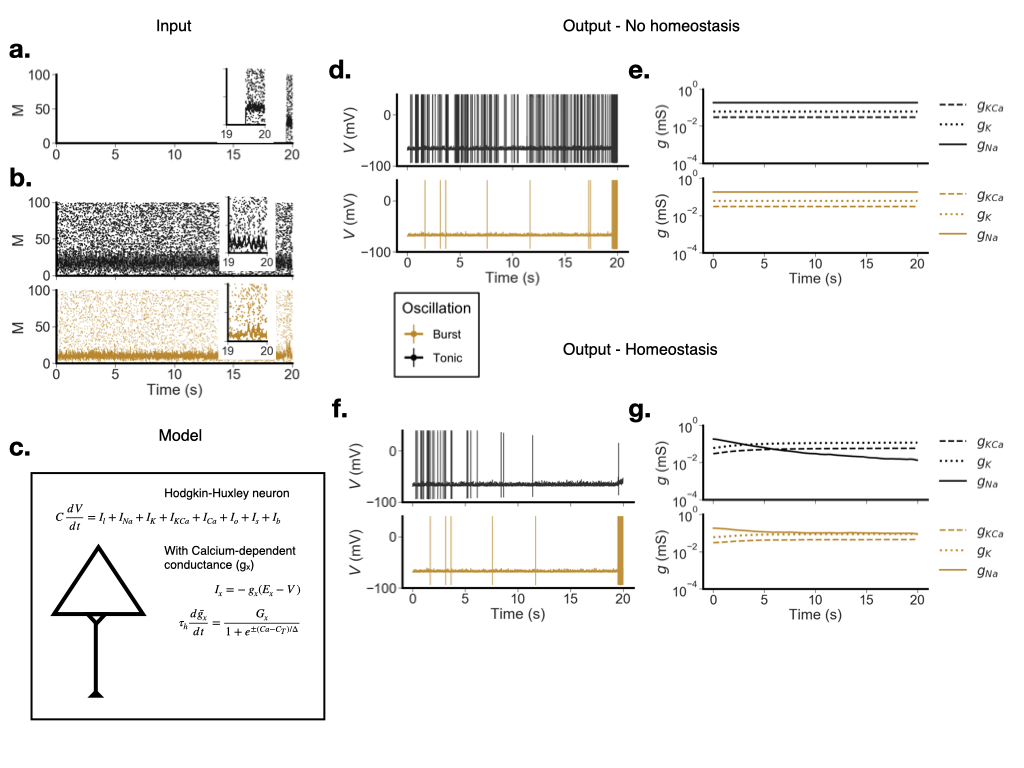
\includegraphics[width=0.9\textwidth]{fig1.png}
\caption{\label{fig:f1}
    Diagram of the model. \textbf{a}. Inputs into the model. Top panel depicts the stimulus, applied over the last 0.5 seconds of each simulated trial. Middle and bottom panels depict the two modes of oscillation we examined: tonic and bursting. 
    \textbf{b}. Illustration of a single model neuron, its major currents, its inputs (top arrow) and its output (bottom arrow).
    \textbf{c.} Examples of model output, including membrane potential (top panel), Ca\textsuperscript{2+} concentration, both observed (solid) and the homeostatic target (dotted line). The bottom panel in c. shows homeostatic dynamics beginning with trial onset, followed by a delay to equilibrium over 20 seconds. Note that there is no homeostatic response to stimulus onset at 19.5 seconds. Also note the log scale on the y axis in this panel.
}
\end{figure}

Note that in real systems intrinsic homeostasis is thought to happen over minutes or days. However, simulation times that are hours or days long are not computationally feasible. So we follow the field and study a model where Ca\textsuperscript{2+} dynamics happen with a 4-second half-life, denoted by $\tau_h$. This might seem like a huge difference. But all that matters mathematically is that Ca\textsuperscript{2+} dynamics happen much slower than all the other synaptic/membrane dynamics. A timescale of $\tau_h > 4$ seconds is a reasonable choice to ensure this. The other major dynamics in the model are synapses with $< 30 ms$ half-lives. This leads to a 133 fold difference \cite{Golowasch1999,Marder2014,Marder2015,Gutierrez2013,Marder2014,OLeary2014,LeMasson1993,Abbott1993}.

% -----------------------------------------------------------------------
\subsection*{Excitatory modulation.}
Homeostasis completely inverts the effect of tonic AMPAergic oscillatory modulation. These excitatory oscillations now result in decreases in both population firing rate, and population synchrony. To see how, first consider how the population responds to a tonic excitatory modulation \textit{without} homeostasis. Without homeostasis, increasing the strength of the excitatory oscillation increases excitability and increases the population firing rate. The action potentials are also grouped by oscillation's rising phase, increasing the population's synchrony (Figure \ref{fig:f2}\textbf{b}, black line). 

With homeostasis this pattern inverts. As excitatory oscillatory modulation strength increases, synchrony and excitability \emph{decreases} (Figure \ref{fig:f2}\textbf{c-d}). Homeostatic mechanisms in the model cause what \emph{should be} excitatory synchronizing modulation to become suppressive and desynchronizing. The stronger the oscillation, the more suppressive the result. By the time the oscillation is about half the strength of the stimulus (which we fix at a firing rate of 6 Hz) the stimulus is completely suppressed and the population firing rate approaches 0 (Figure \ref{fig:f2}\textbf{c}).

We compared the effect of tonic oscillation to short 4-cycle bursts of excitatory modulation, presented only during the stimulus. Here, the oscillation period is far too short to provoke homeostasis. This means that increases in oscillatory strength continue to increase population firing rate and synchrony (Figure~\ref{fig:f2}\textbf{e} and \textbf{f}).

Of course theta oscillations in hippocampus are GABAergic, not AMPAergic as we model here. Exploring this artificial oscillation lets us show the central principle we want to highlight in our simple model. It seems that tonic oscillations--when joined with homeostasis--can profoundly alter the coding properties of what one would expect from oscillatory modulation. The degree of effect depends on the degree to which the oscillation changes the cell's tonic Ca$^{2+}$. It also shows that because of homeostasis, bursts are \textit{qualitatively distinct} from their tonic counterparts.  

The specific effect we observed (suppression of excitability) is seen because the homeostatic equations that \textit{we chose} respond to changes in Ca\textsuperscript{2+} by decreasing the conductance of the Na and Ca channels, and increasing the conductance of K and KCa channels (Eq~\ref{eq:dgdt}). The net effect of these dynamics is to decrease the sodium channel conductance, and increase the potassium. This makes firing an action potential less likely, for any given input. These channel dynamics are visualized in Figure~\ref{fig:f1}\textbf{c} and the corresponding FI curve is shown in Figure~\ref{fig:f4}. 

The general effect we would expect for some other selection of channels, chosen by some other theorists or by evolution itself, depends on those channels. O'Leary \cite{OLeary2014} has shown how complex the relationship is between homeostasis, channel conductance, and neuronal firing patterns. It's complex enough that general statements are probably impossible. On the one hand, our simple model has been shown by others to recapitulate hippocampal pyramidal cell's activity in laboratory settings \cite{LeMasson1993}. On the other, it is \textit{very simple} and so most probably incomplete at best. Experimental testing is needed. 

Note that the inversion in Kappa seen in Figure~\ref{fig:f2}\textbf{d} as well as in \ref{fig:f5}\textbf{b}, is the result of the decrease in excitability. Put another way, it's a low $N$ effect. As population spiking is suppressed, the total number of spikes declines to the point where the bins used to calculate the Kappa correlation often contain no spikes. This leads to a somewhat misleading increase in synchrony.

\subsection*{Inhibitory modulation.}
GABAergic oscillatory modulation does not lead to a homeostatic response in our model. This is true for both tonic oscillations and bursts. In all cases, as oscillatory strength increases, population firing declines dramatically (grey lines in Figure \ref{fig:f2}\textbf{a-d} and light yellow lines in panel \textbf{e-f}).

\begin{figure}
\centering
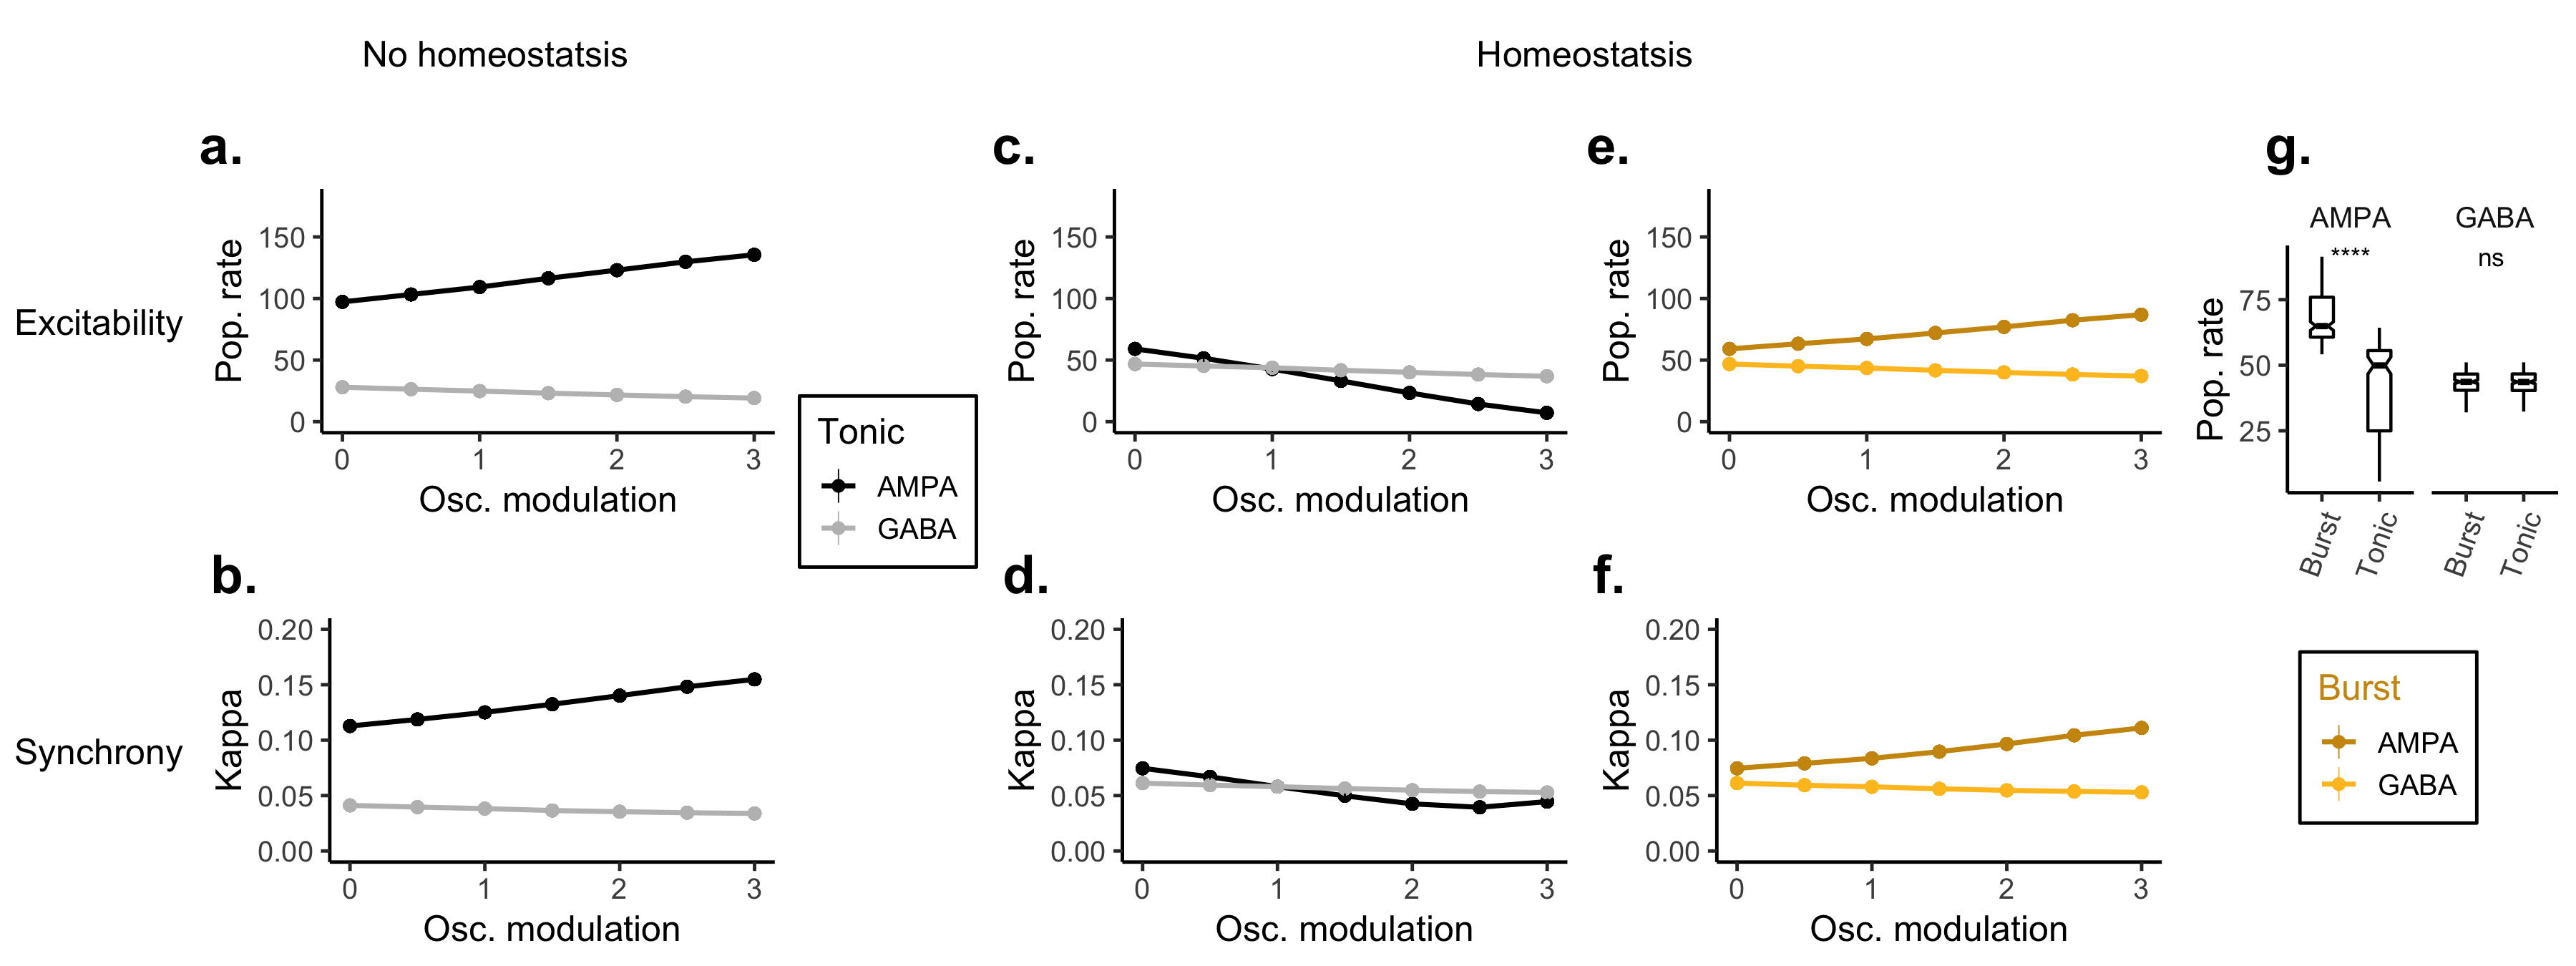
\includegraphics[width=1\textwidth]{fig2.png}
\caption{\label{fig:f2}
    The effect of oscillatory modulation on synchrony--which is measured using the Kappa correlation (Eq~\ref{eq:kappa})--and excitability, measured by the population firing rate. Tonic oscillations are shown in grey and black. Bursts are shown in light and dark yellow.
    \textbf{a.}-\textbf{b.} Increases in tonic modulation strength, without homeostasis. This is our reference condition. Top panel (a.) is the observed population firing rate averaged over the 0.5 second stimulus. Bottom (b.) is synchrony over the same period.
    \textbf{c.}-\textbf{d.} Same experiment as a-b but with Calcium-mediated homeostasis, showing how homeostasis with tonic AMPA oscillations reduces population firing and synchrony.
    \textbf{e.}-\textbf{f.} Burst modulation, presented during the stimulus period (4 cycles of oscillation, onset time: 19.5 s).
    \textbf{g.} Change in excitability between bursts and tonic rhythms for all oscillation firing rates. Asterisks denote a significant difference using the Wilcoxon rank sum test ($W = 1886.5, p < 2.2e-16$). The frequency of the oscillatory rhythm was fixed at $f = 8$ in all models.}
\end{figure}

In Figure~\ref{fig:f2} we compared AMPA and GABAergic models of the theta rhythm (8 Hz). This is done to illuminate their differences, but is not biologically realistic. Physiological theta is a GABAergic. AMPAergic oscillations of the hippocampus are, however, seen in the high gamma range (60-90 Hz). In Figure~\ref{fig:f3} we confirm AMPAergic oscillations in this range follow the same pattern as theta. For both 60 and 90 Hz gamma, tonic oscillations suppress excitability and desynchronize firing.

\begin{figure}
\centering
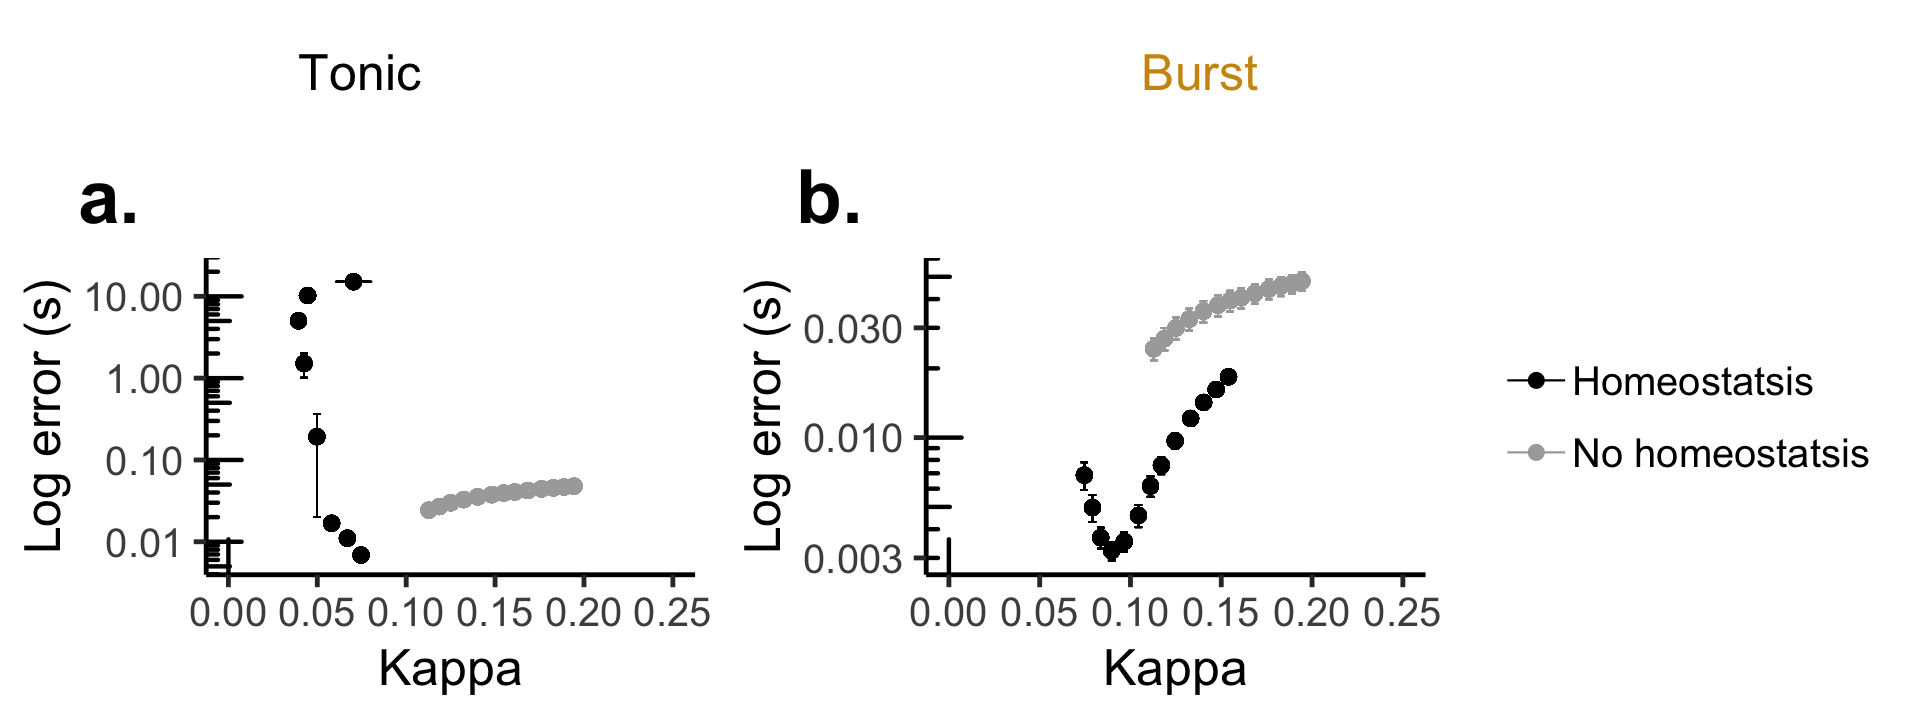
\includegraphics[width=0.5\textwidth]{fig3.png}
\caption{\label{fig:f3}
    The effect of fast AMPAergic gamma oscillations for both tonic oscillation and 4-cycle bursts. 
    Top panel (\textbf{a}.) is the observed population firing rate averaged over a 0.05 second or 0.033 second stimulus. Bottom (\textbf{b}.) is synchrony over the same period. Columns in both \textit{a.} and \textit{b.} represent with 60 or 90 Hz gamma. The stimulus window was matched to the length of time 3 cycles of oscillation would take.
}
\end{figure}

\subsection*{Homeostasis and excitability.}
In our model Ca\textsuperscript{2+} influx is driven by increases in the membrane voltage, and Ca\textsuperscript{2+} concentration is restored both by a passive and linear recovery (Eq~\ref{eq:passive}) and active homeostasis (Eq.~\ref{eq:dgdt}). Homeostasis works by negative feedback. Increases in Ca\textsuperscript{2+} concentration decrease the conductance of both the sodium and potassium channels in our model (Eq.~\ref{eq:HHH}). This decrease in conductance in turn lowers the membrane voltage down closer to its resting value. As the voltage falls so does the Ca\textsuperscript{2+} concentration. The excitability changes we see with homeostasis must be due to the decrease in Na conductance. Changes due to K conductance--which acts to recover the voltage following a spike--can't alter baseline.

One the simplest, classic ways to measure the excitability of a cell--simulated or real--is with an FI-curve. In an FI-curve a small square wave of current is injected into the cell, and the resulting increase in firing rate (if any) is averaged over a short window. In Figure~\ref{fig:f4} we show the average FI-curve for 100 simulated hippocampal neurons. Under homeostasis the FI-curve is lower, which means there has been a substantial suppression in the membrane excitability.

\begin{figure}
\centering
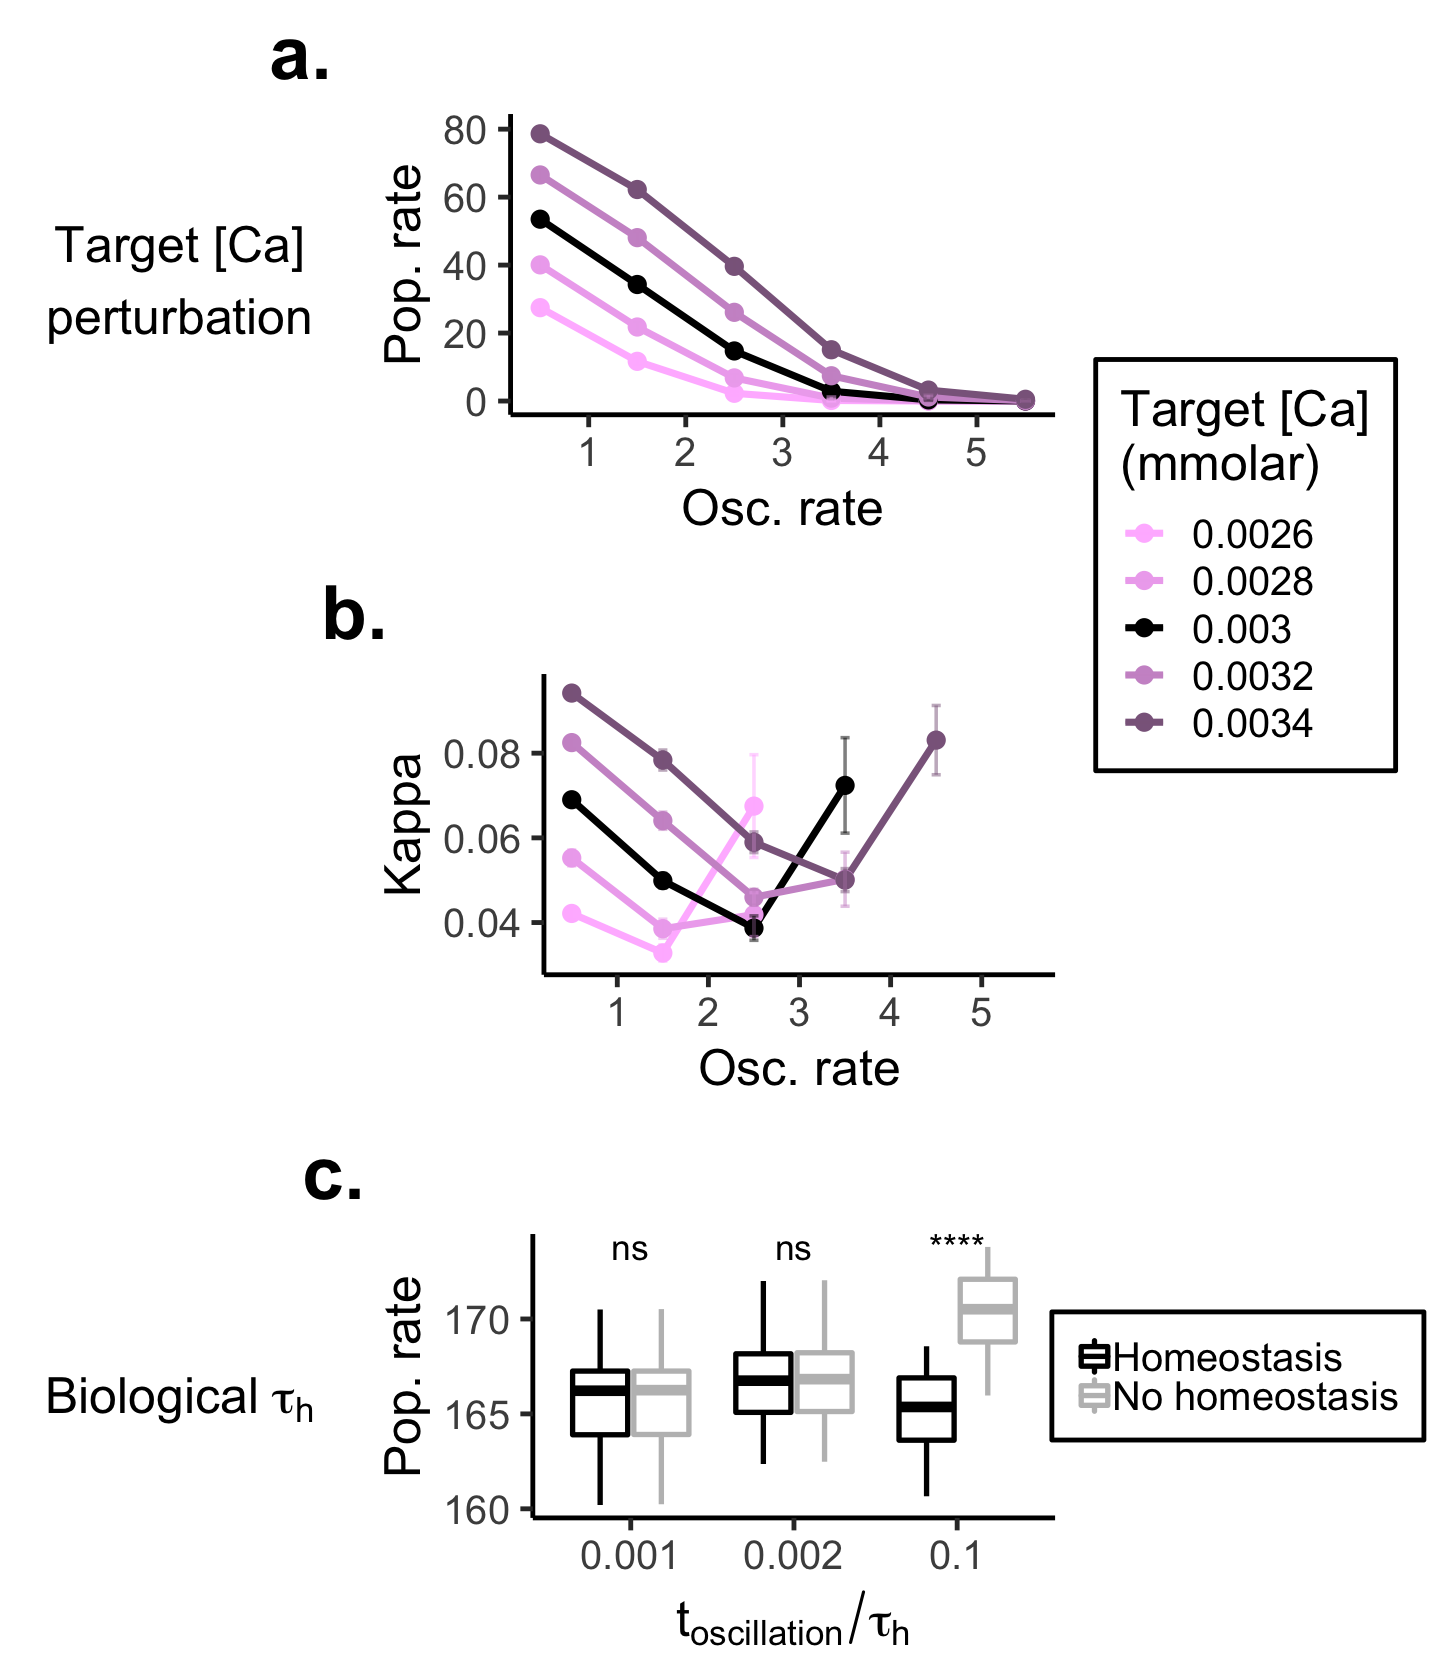
\includegraphics[width=0.4\textwidth]{fig4.png}
\caption{\label{fig:f4}
Excitability and homeostasis. An average FI-curve for 100 hippocampal neurons, with (black) and without (grey) homeostasis. In both models, oscillation was tonic and AMPAergic. The square-wave pulse lasted 0.1 seconds, and ranged from 0.1 to 1 $\mu$amps, sampled every 0.01 $\mu$amps.
}
\end{figure}

% -----------------------------------------------------------------------
\subsection*{Controls and perturbations.}
To ensure our parameter choices in the model were generalizable, we perturbed several key values by 10-20 percent.

When the model is run with only stimulus-driven homeostasis, the Ca\textsuperscript{2+} concentration equilibrates to about 0.003 mM. We used this as a standard target value for all modulation experiments, until now. When we vary this value in 0.0002 mM increments, population rate and synchrony either increases or decreases depending on whether the Ca\textsuperscript{2+} increases or decreases, shown Figure \ref{fig:f5}\textbf{a-b}. However despite different initial Ca\textsuperscript{2+} concentrations, each model still shows an identical set of trends as the strength of the oscillation increases (Figure \ref{fig:f5}). That is, increasing or decreasing the target concentration shifts the overall excitability of the population, in an approximately linear way. This means that while the initial choice of 0.003 mM was arbitrary, the qualitative pattern of results we report is not dependent on this choice.

We chose a 4-cycle length for bursts somewhat arbitrarily. Real oscillations range in duration from single cycles to seconds of even minutes \cite{Lundqvist2016,vanEde2018}. Our burst/tonic distinction is therefore a false (but useful) dichotomy. To find a better estimate of how an oscillation would need to last, on average, to generate a homeostatic response we ran some long simulations using a more realistic homeostatic time constant ($\tau_h$ = 600 seconds; up from 20 seconds). It seems an oscillation would need to be present \textit{at least} 10\% of the time to generate a response (Figure~\ref{fig:f5}\textbf{c}). 

Real theta rhythms drift in frequency \cite{Buzsaki2015}. To test if small differences in frequency have a notable effect, we simulated small drifts in frequency of theta ranging from 6-10 Hz. Frequency drift had no visible effect on the homeostatic suppression of excitability (Figure~\ref{fig:f5}\textbf{d}-\textbf{e}).

The leak conductance ($g_L$, Eq.~\ref{eq:HHH}) plays a key role in setting the resting potential of the cell. The resting potential in turn helps determines overall membrane excitability, and sets the resting Ca\textsuperscript{2+} concentration. This means our Ca\textsuperscript{2+} set point (of 0.003 mM) depends on the $g_L$ in practice but our choice of of 0.003 mM was arbitrary. To test if a small mis-match between $g_L$ and the set-point altered our results, we ran several experiments perturbing the leak conductance while keeping the Ca\textsuperscript{2+} set-point fixed. Changes to leak conductance had only a small effect on homeostasis (Figure~\ref{fig:f5}\textbf{f}-\textbf{g}).

\begin{figure}
\centering
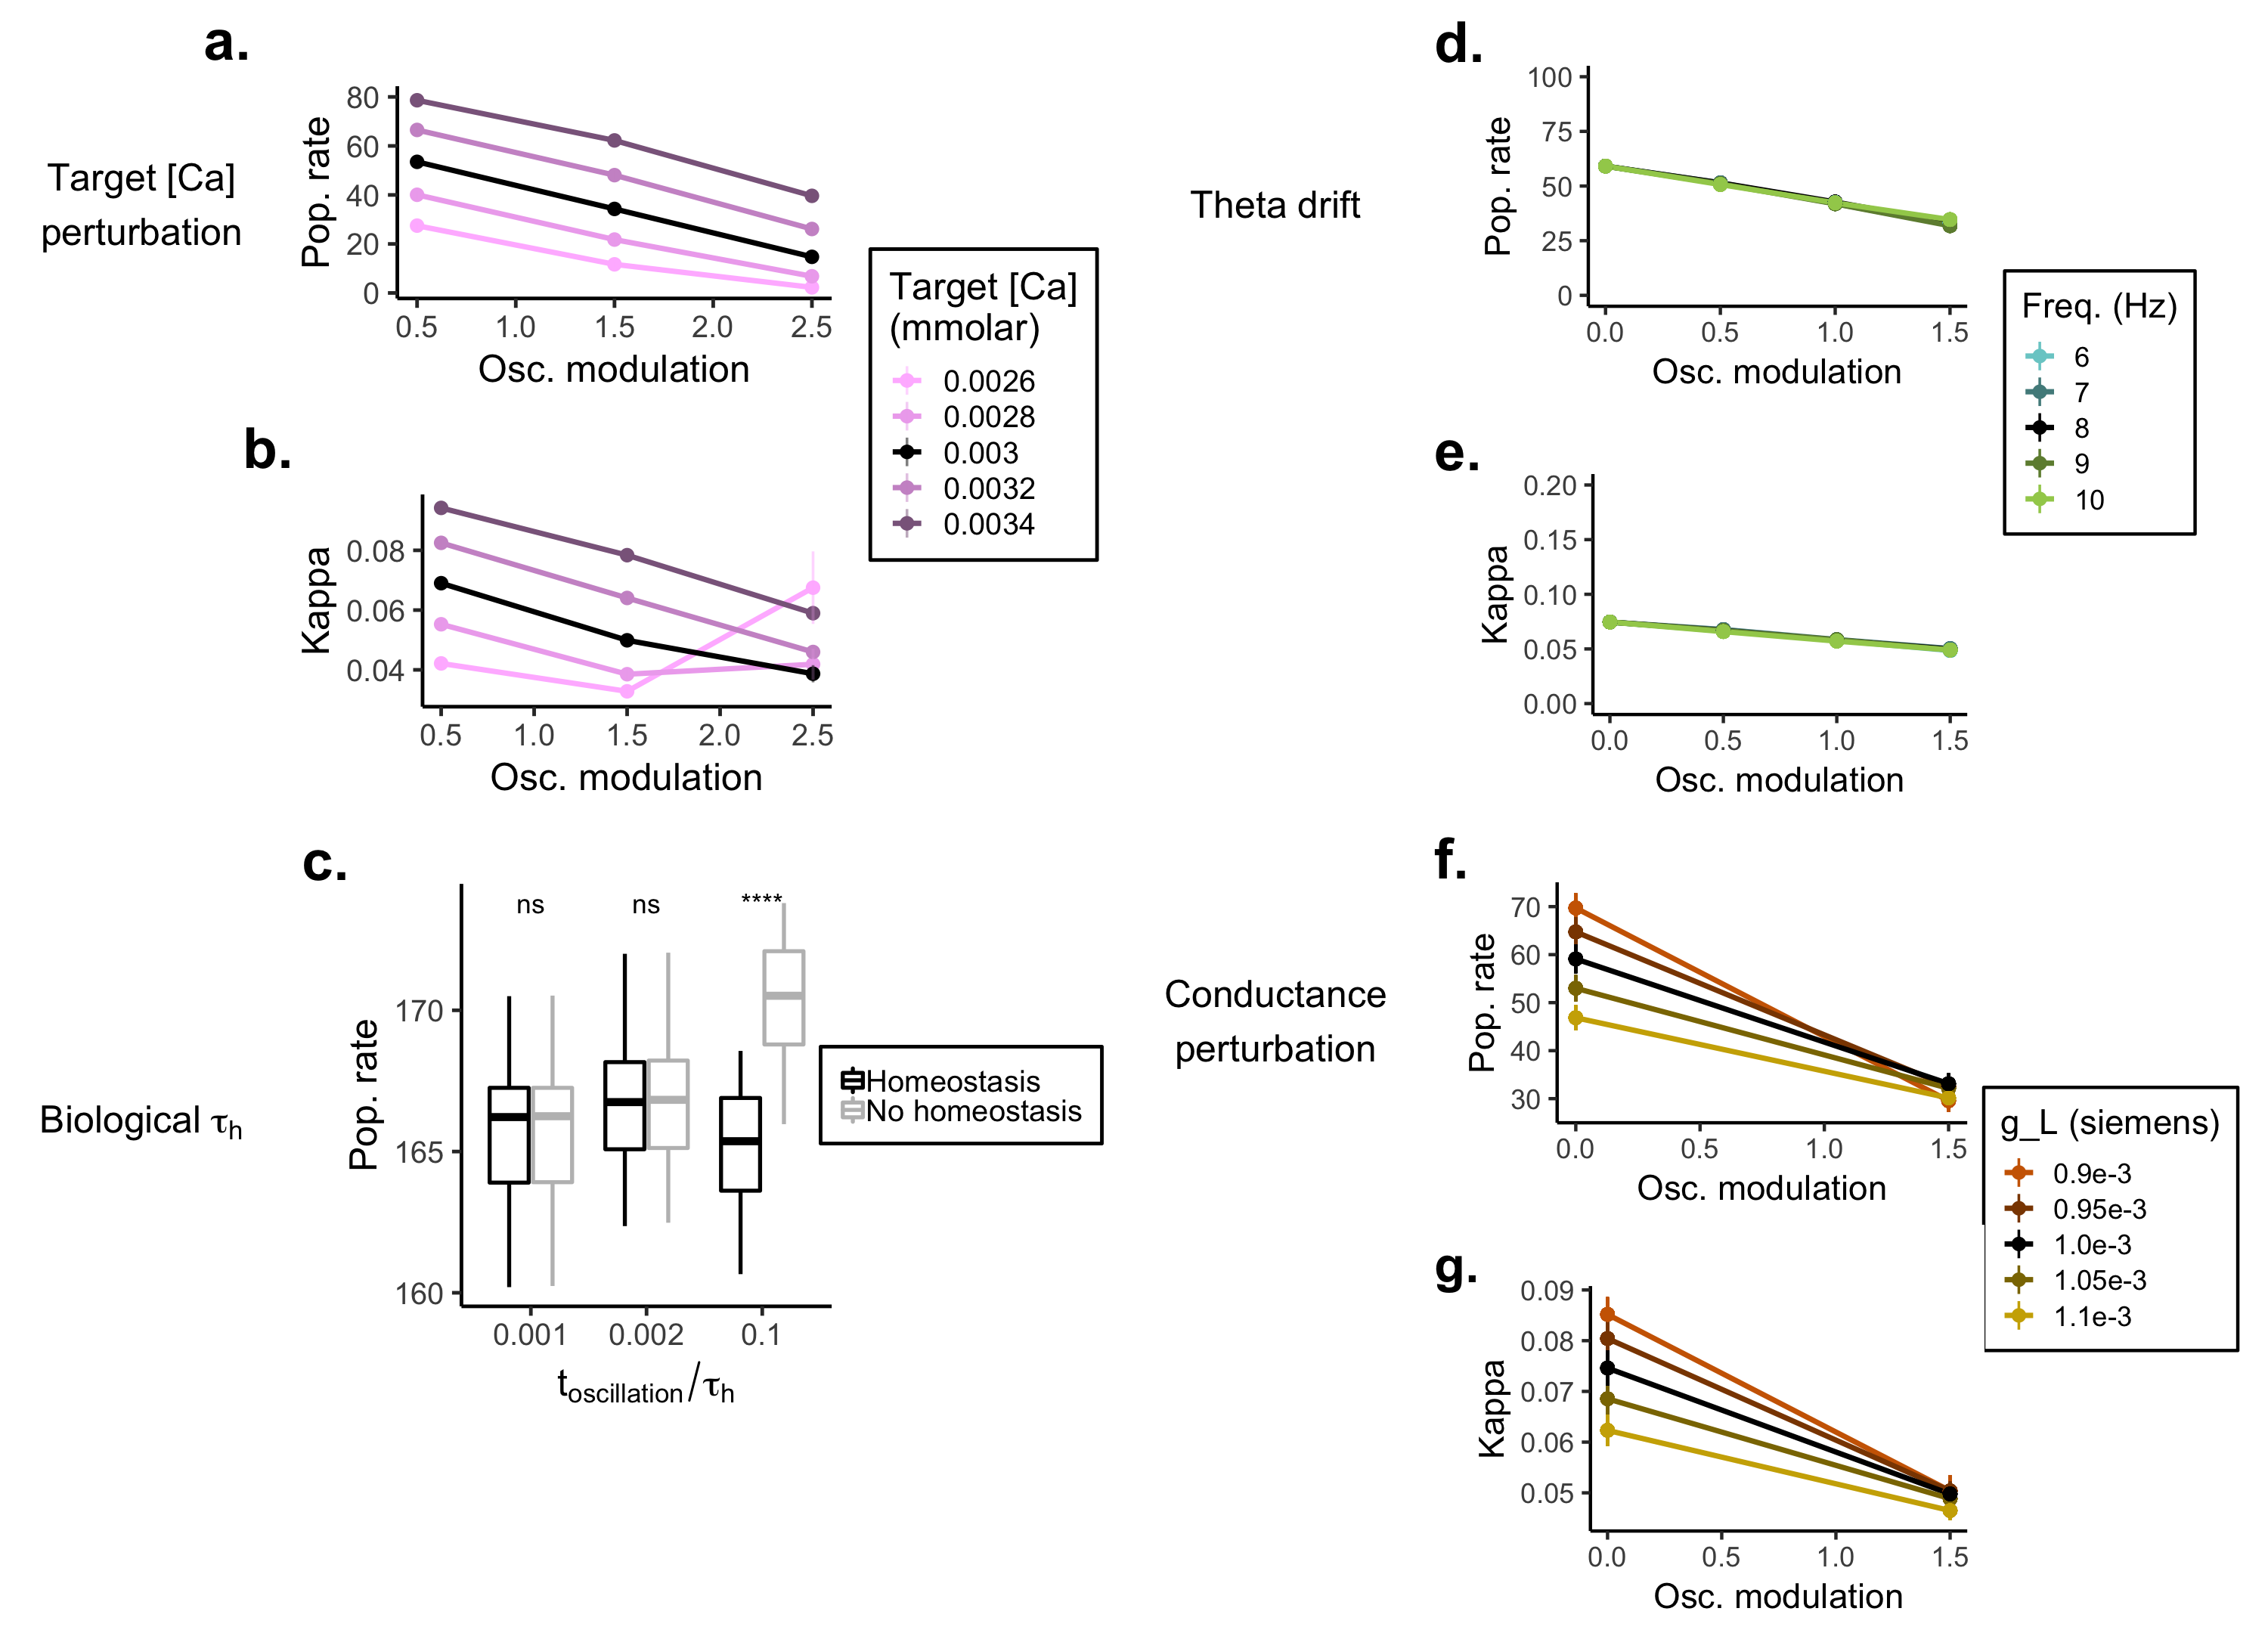
\includegraphics[width=1\textwidth]{fig5.png}
\caption{\label{fig:f5}
    Control experiments.
    \textbf{a.} Change in population hippocampal population rate for different levels of target [Ca] (colors) as a function oscillation strength (Osc. rate on the x-axis). All values are referenced to a no-modulation control.
    \textbf{b.} Change in population synchrony for different levels of target [Ca] (colors) as a function oscillation strength (firing rate). All values are referenced to a no-modulation control.
    \textbf{c.} Change in population rate as the oscillation duration approaches a more realistic $\tau_h$, the half-life of the homeostasis dynamics (Eq.~\ref{eq:dgdt}). In this control experiment we used a more biologically realistic $\tau_h$ of 600 s (or 10 minutes). All other simulations in the report use a $\tau_h$ of 4 seconds, which is well below most reports of this value in real systems. However in choosing such as small value we follow the majority of the homeostasis modeling literature (for more on this see the \textit{Discussion}).
    \textbf{d}.-\textbf{e}. The effect of frequency drift (see legend) on homeostasis with tonic AMPAergic modulation.
    \textbf{f}.-\textbf{g}. The effect of altering the leak conductance ($g_L$) on homeostasis with tonic AMPAergic modulation.
}
\end{figure}


% -----------------------------------------------------------------------
% -----------------------------------------------------------------------
% -----------------------------------------------------------------------
\section*{Discussion}
Our scientific understanding of homeostasis has been shaped as much by theoretical work as empirical \cite{Marder2014}. In an attempt to understand the interaction between oscillatory modulations and homeostasis, we begin by studying one of the simplest models used in early studies of homeostasis--a population of point neurons in the hippocampus \cite{LeMasson1993}.

Our simple models offer answers to three basic questions. One, do tonic oscillations engage homeostatic mechanisms? Two, does homeostasis in turn change the oscillation's function? Three, do short bursts of oscillation have distinct effects from tonic oscillations? Put another way: can homeostasis explain why some oscillations, such as hippocampal theta, tend to appear as tonic rhythms while other oscillations (like those in cortex) tend to appear as bursts? 

Homeostasis is generally viewed as a stabilizing force. This is the goal of homeostasis in our model as well. However oscillatory modulation is a unique form of modulation; It shares neurotransmitters, and even synapses, with non-modulatory stimuli. As a result, homeostatic corrections for modulation must affect both the modulator and the driver \cite{Sherman1998}. Our work suggests this trade-off can be quite strong. To avoid this trade-off, sometimes anyway, we speculate that the long-time scale of evolution may favor different types of oscillation for different functional roles. 

Bursting, rather than sustained, oscillations tend to be common in the cortex. One striking example is in motor cortical regions, where beta (~12-30 Hz) bursts are prevalent and likely functional. Specifically, beta bursts are very short--sometimes lasting only one or two cycles \cite{Sherman2016}--and relate to self-timed movements \cite{Feingold2015}. Patients with Parkinson's disease show increased motor rigidity and bradykinesia, symptoms associated with prolongation of beta bursts \cite{Tinkhauser2017}. Levodopa treatment was shown to decrease burst probability and duration, and that decrease in burst duration correlated with motor improvement \cite{Tinkhauser2017}.

An important counterexample to beta is visual cortical alpha (8-10 Hz). Alpha is tonic and high powered when humans rest with their eyes closed. Even though both cortical and sub-cortical alpha generators are synaptically excitatory, this rhythm has however been associated with suppression of excitability \cite{Jensen2002,Bonnefond2012,Peterson2017}. While several competing explanations have been offered \cite{Bonnefond2012,Lange2013,Peterson2017} for this, our work raises another possibility that is complementary to the others. Specifically, though we modelled hippocampal cells, the same Ca\textsuperscript{2+} homeostatic mechanisms exist in visual cortex (and the neocortex as a whole). This means that strong and tonic alpha oscillations, combined with homeostasis, should directly suppress population firing in visual cortex. Such an effect, were it to occur, would last well past the moment of oscillation offset. In fact, such long term effects of alpha have been reported in the literature \cite{Jensen2002,Bonnefond2012}, though the physiological mechanism was often unclear. Our work suggests that intrinsic homeostasis may underlie this effect.

\subsection*{Limitations}
The nature of our model--the fact that we use point neurons with only 6 currents--or the fact that our model is strictly feed-forward--without lateral or recurrent connections--means we don't know with confidence to what degree our model's effects will appear in more complex models, or in real neural systems. O'Leary \citep{OLeary2014} and others have shown how exceptionally complex the homeostatic response is. It is therefore likely some neurons will have a homeostatic response that is nothing like that in our model. Others may be naturally immune to oscillatory effects. There may be many such examples.

We do know, however, that oscillations are a ubiquitous feature of cortical activity, as is Ca\textsuperscript{2+}-mediated intrinsic homeostasis. This means the ingredients for oscillation and homeostasis to interact are omnipresent in both sub-cortical and cortical areas. This response might be very different than what we found. But that there could be broad range of effects makes our initial results in a simple model all the more intriguing. 

The basic mechanisms of Ca\textsuperscript{2+}-mediated intrinsic homeostasis are conserved across phyla \cite{Tran2017}. Meaning the qualitative properties of our model may also be present across phyla. That said the mechanisms for homeostatic interactions, along with their quantitative properties, depend on a number of factors specific to each cell and circuit. These include the duty cycle, power, and frequency of an oscillation, as well as on synaptic strengths and their location in the dendritic tree (an idea we return to below). It also depends on the other inputs into the cell, both from fast synaptic transmission and other (slower) modulators, as well a connection type; simulation studies suggest that recurrent connections can strongly interact with homeostatic regulation \cite{Harnack2015}. The temporal and spatial scales of these factors will strongly influence Ca\textsuperscript{2+} dynamics, which is in turn central to governing what, if any, homeostatic effects oscillations may generate.

We did not study synaptic homeostasis. Synaptic homeostasis can also play key a role in combating oscillatory perturbations \cite{Cannon2016}. There is some evidence intrinsic homeostasis appear to be linked excitatory synaptic homeostasis \cite{Joseph2017}. Still, the exact nature of the homeostatic response depends on how, and to what degree, oscillatory and other sensory or internally driven inputs share synapses. This, in turn, requires considering complex dendritic arbors and their effect on homeostasis \cite{LeMasson1993}, neuromodulation \cite{Jadi2012,Jadi2014}, and computation \cite{Mainen1996,Polsky2004,Mel2004}. Considering these interacting effects together is the next step needed to develop a clearer biological understanding of modulatory oscillations. For inhibitory oscillations the case is even more complex: Ca\textsuperscript{2+} in these cells does not appear to regulate intrinsic homeostasis, but synaptic homeostasis is under a separate mechanism of control \cite{Joseph2017}.

\subsection*{Previous work}
Homeostasis has been extensively studied in the rhythmic pacemaker present in the crab stomatogastric ganglion. Here homeostasis has been shown to stabilize self-organized oscillations \cite{Golowasch1999}, and interact with neuromodulation in a \textit{highly} state dependent way \cite{Marder2014,Marder2015,Marder2014}. Like our model though the oscillation present in the STG is tonic. This means it could in principle drive a second homeostatic response. However, synapses in the stomatogastric ganglion circuit are predominately inhibitory \cite{Marder2015}. If our model predictions held up for this circuit we would expect there to be no second response.

The interaction between homeostasis and oscillations has previously been considered in a simple model of cortex. But the oscillatory input here was treated as a signal, not a modulator. Cannon and Miller \citep{Cannon2017} explored how synaptic homeostasis can effectively minimize the effect of modulatory perturbations, thus maximizing mutual information between an incoming oscillatory signal and a single cell's firing pattern. Our analysis could be considered an inverse complement to \citep{Cannon2017}--we study how to minimize the perturbation caused by a modulatory oscillator, rather than how to maximize the transmission of an oscillator.

\subsection*{Conclusion}
 Here, using a relatively simple model of hippocampal neurons, we observe a surprising--even paradoxical--result: that homeostatic effects can invert a normally synchronizing excitatory oscillatory neuromodulator and cause it to become inhibitory and desynchronizing.
 
 If our simple model is right, we conjecture that intrinsic homeostasis can explain why tonic theta rhythms in the hippocampus are synaptically inhibitory. To make this clear, consider the alternative. If the theta rhythm was strong, tonic, and synaptically excitatory, our model suggests this could lead to an equally strong--but opposing--homeostatic response. Such a response can mean that sodium conductance decreases, which in turn decreases the likelihood a hippocampal neuron could respond to any given stimulation. 

In effect, the homeostatic response to strong excitatory oscillations consumes a substantial portion of each cell's dynamic range. On the other hand, inhibitory oscillations--which do not generate an intrinsic homeostatic response--leave the dynamic range of neurons intact. This may also explain why neocortical oscillations tend to be short and bursty, and why some neurological disorders, such as Parkinson's disease, are associated with prolonged excitatory rhythms.

% Computational modeling plays a critical role in neuroscience. Explicit computational modeling moves the field from "word model" theories to self-consistent mathematical formalizations [REF]. While these models can be wrong, they offer testable novel venues for research that are often difficult to find due to the immense complexity of the rich, dynamic neuronal environment.

\section*{Methods}
\subsection*{Mathematical model}
We model an unconnected population of hippocampal neurons, subjected to oscillatory modulation. This is instantiated as $N = 1000$ input cells connected to $M = 100$ Hodgkin-Huxley neurons. The $M$ cells in the population were tuned to mimic regular firing \cite{Borgers2005,Borgers2008}. The firing pattern of each input cell (both stimulus and modulation) is from a Poisson process, with a time-varying rate. $N_o$ cells oscillate. $N_s$ serve as input. For simplicity, we let $N_o = \frac{N}{2}$ so $N_o = N_s$. All input cells have a $p = 0.1$ connection probability to the hippocampal population. The hippocampal population has no lateral of recurrent connections. The synaptic weights for all $N \rightarrow M$ connections $w$ were independently sampled from a uniform distribution, $w \sim \mathcal{U}(5, 50)$ $\mu$S. The firing rate of the oscillating population was governed by sinusoidal pacemaker, with amplitude $A$ and frequency $f$, with the exact form $\frac{r_o}{2} (1 + \text{sin}(2 \pi f t))$. As a result, $r_o$ defines the peak firing of the oscillation. The stimulus population was simply modeled by a fixed rate of 6 Hz ($r_s$). 

Hodgkin-Huxley dynamics were governed by 4 active ionic currents ($I_{Na}$, $I_{K}$, $I_{KCa}$, $I_{Ca}$) and the passive leak current ($I_l = g_l (E_l - V)$). Besides $I_{Ca}$ (which is discussed below), active currents are governed by the standard Hodgkin and Huxley form \cite{Hodgkin1952}. Where $m$ and $h$ respectively track the opening and closing channel kinetics, $p$ and $q$ are channel dependent parameters, and $V_i$ is the channel appropriate Nernst reversal potential. See \textit{Table 1} for the complete set of parameters.

\begin{equation}
\label{eq:Idef}
I = \bar{g} m^p h^q (V_i - V)
\end{equation}

The Ca\textsuperscript{2+} current $I_{Ca}$ was governed by a form taken from the Morris-Lecar model \cite{Morris1981,LeMasson1993,Siegel1994}.

\begin{equation}
I_\text{Ca} = g_\text{Ca} [1 + \text{tanh} \Big ( \frac{V_1 - V}{ V_2} \Big ) (V_\text{Ca} - V)]
\end{equation}

Overall membrane dynamics were governed by these internal ion conductances, a variable bias current $I_\text{bias}$, and the excitatory synaptic input term $I_S$, which contains both stimulus and oscillatory terms. All synaptic input was in turn governed a single exponential kinetics, which we denote generically using an $x$ subscript below. Though each synaptic input had different inputs, all models shared the same parameters. That is, $\tau_x = \tau_b = \tau_s = \tau_o$ and $\bar{g_x} = \bar{g_b} = \bar{g_s} = \bar{g_o}$.

\begin{equation}
    I_S = -g_s (V_e - V) + -g_o (V_o - V) 
\end{equation}
\begin{equation}
    \tau_x \frac{dg_x}{dt} = -g_x + \bar{g_x} \delta(t - t_x^j)
\end{equation}

\begin{equation}
\label{eq:HHH}
C \frac{dV}{dt} = I_l + I_{Na} + I_{K} + I_{KCa} + I_{Ca} + I_{\text{bias}} + I_{S} 
\end{equation}

The intrinsic excitability is regulated by altering both inward and outward conductances in response to changes in Ca\textsuperscript{2+} concentration. Following the previous work \cite{LeMasson1993} and \cite{Siegel1994}, we modeled this by allowing the maximal conductances $\bar{g_\text{Na}}$, $\bar{g_\text{K}}$, $\bar{g_\text{KCa}}$, and $\bar{g_\text{Ca}}$ to non-linearly vary in response to changes in Ca\textsuperscript{2+} concentration, $\text{Ca}$. During homeostatic equilibration, conductances drifted until the target Ca\textsuperscript{2+} concentration was met, denoted as $C_T$. In a control experiment a range of $C_T$ values were explored (Figure \ref{fig:f5}), though simulations default to 0.03 mM; the value the system reaches with stimulation ($r_s = 6$ Hz) without modulation ($r_o = 0$). The $\pm$ symbol in equation \ref{eq:dgdt} denotes the direction of ion flow and is $(+)$ for inward going currents (Na and Ca) and $(-)$ for outward going Potassium.

\begin{equation}
\label{eq:dgdt}
\tau_h \frac{d \bar{g_x}}{dt} = \frac{G_x}{1 + e^{\pm (Ca - C_T)/\Delta}}
\end{equation}

Ca\textsuperscript{2+} dynamics were assumed to follow first order kinetics, driven by the Ca\textsuperscript{2+} influx current and clearance rate constant $k$. Values for both $\gamma$ and $k$ were taken from \cite{Liu1998}.

\begin{equation}
\label{eq:passive}
\frac{d\text{Ca}}{dt} = -k \text{Ca} - \gamma I_\text{Ca}
\end{equation}

% \subsection*{Estimating excitability, synchrony, and error}
\subsection*{Estimating excitability and synchrony}
We measure excitability by comparing average firing rate of all $M$ neurons in an experiment, with ($r_m$) and without modulation ($\bar{r}_m$). 

\begin{align}
    \label{eq:excite}
    \Delta r = \bar{r}_m - r_m
\end{align}

We measure synchrony using $\kappa$, a binned measure of spiking covariance \cite{Wang1996}. Where $X(l) = 0 \ \text{or} \ 1$ and $Y(l) = 0 \ \text{or} \ 1$ for $l = \{1, 2, ..., K \}$ and with $T/K = \tau$.

\begin{align}
    \label{eq:kappa}
    \kappa_{ij}(\tau) = \frac{\sum_l^K X(l)Y(l)}{\sqrt{\sum_l^K X(l) \sum_l^k Y(l)}}
\end{align}

\begin{align}
\kappa(\tau) = \frac{1}{N} \sum_i^N \sum_j^N \kappa(\tau)_{ij}
\end{align}

% Modulation is optional. Each of the different modulatory systems--oscillations, dopamine, and acetylcholine--to name a few among dozens of options, may be absent, weakly present, or operating at high level at any given moment of time. We therefore reason it is important to quantify how coding is perturbed under varying levels of modulation and homeostasis. We estimate this by comparing differences in spike timing between an experimental condition and a control run with without modulation. 

% Deviations in spike-timing caused by modulation are treated as errors, which we quantify with the mean squared error (Eq.~\ref{eq:error}). The more efficient a modulation, the less error it should introduce for a given change in either excitability or synchrony.  

% \begin{equation}
% \label{eq:error}
% \text{MSE} = \frac{1}{K} \sum_{i=1}^k (\hat{y} - y_i)^2
% \end{equation}

% In its mathematical form the MSE assumes the reference $\hat{t}$ and observed variables $y$ to be the same length. Here this constraint could not be satisfied: as $r_o$ increases, new action potentials are inevitable. To accommodate potentially ragged lengths we truncated the longer of the two series to match the shorter. For example, if the target series has length $K$, and the observed sequence has length $L$, when $K > L$ then $K-L$ elements are removed, starting with the largest value. When $L > K$, $L - K$ of the largest were eliminated. 

% -------------------------------------
\newpage
\begin{table}
\centering
\begin{tabular}{@{}lll@{}}
\toprule
\textbf{Symbol} & \textbf{Range (unit)} & \textbf{Description} \\ \midrule
$f$ & 8 (Hz) & Oscillation frequency \\
$r_o$ & 0 - 6 (Hz) & Oscillation firing rate \\
$r_s$ & 6 (Hz) & Stimulus firing rate \\
$C$ & 1 ($\mu$F) & Membrane capacitance \\
$\tau_h$ & \textgreater 4 (sec) & Homeostasis time constant \\
$w$ & 5 - 50 ($\mu$S) & Synaptic weight \\
$\tau_e$ & 5 (msec) & Excitatory synaptic time constant \\
$V_e$ & 0 (mV) & Excitatory synaptic reversal potential \\
$V_i$ & -80 (mV) & Inhibitory synaptic reversal potential \\
$p$ & 0.1 & Connection probability (stimulus, modulation) \\
$C_T$ & 0.0028-0.0032 (mM) & Target Ca\textsuperscript{2+} concentration \\
$G_\text{Na}$ & 360 ($\mu$S) & Initial Na conductance \\
$G_\text{K}$ & 120 ($\mu$S) & Initial K conductance \\
$G_\text{KCa}$ & 60 ($\mu$S) & KCa conductance \\
$g_\text{Na}$ & 180 ($\mu$S) & Max. Na conductance \\
$g_\text{K}$ & 60 ($\mu$S) & Max. K conductance \\
$g_\text{KCa}$ & 30 ($\mu$S) & Max. K conductance \\
$g_\text{Ca}$ & 0.03 ($\mu$S) & Max. Ca\textsuperscript{2+} conductance \\
$g_l$ & 1 ($\mu$S) & Leak conductance \\
$V_l$ & -70 (mV) & Leak reversal potential \\
$V_K$ & -100 (mV) & K reversal potential \\
$V_\text{Na}$ & 50 (mV) & Na reversal potential \\
$V_\text{Ca}$ & 150 (mV) & Ca\textsuperscript{2+} reversal potential \\
$V_\text{1}$ & -50 (mV) & Morris-Lecar constant \\
$V_\text{2}$ & 10 (mV) & Morris-Lecar constant \\
$\Delta$ & 0.6 ($\mu$M) & Ca\textsuperscript{2+} influx rate \\
$k$ & 1/200 (1 / msec) & Ca\textsuperscript{2+} clearance rate \\
$\gamma$ & -0.00047 (mM / mA / msec) & Ca\textsuperscript{2+} current conversion constant \\
$\delta t$ & 0.01 (msec) & Integration time step \\ \bottomrule
\end{tabular}
\caption{Model parameters.}
\label{table:params}
\end{table}

% -----------------------------------------------
\newpage
\bibliography{library_min}

% -----------------------------------------------
\end{document}
